\documentclass[11pt,letterpaper,oneside]{report}
\usepackage[T1]{fontenc}
\usepackage[utf8]{inputenc}
\usepackage[english]{babel}
\usepackage{lmodern}
\usepackage{microtype}
\usepackage[margin=0.86in,headheight=16pt]{geometry}
\usepackage[table,dvipsnames]{xcolor}
\usepackage{graphicx}
\usepackage{booktabs,tabularx,longtable,array}
\usepackage{enumitem}
\usepackage{titlesec}
\usepackage{fancyhdr}
\usepackage{hyperref}
\usepackage{xurl}
\Urlmuskip=0mu plus 1mu\relax
\usepackage{tcolorbox}
\usepackage{listings}
\usepackage{tikz}
\usetikzlibrary{arrows.meta,positioning,shapes.geometric,fit,calc}
\usepackage{needspace}
\usepackage{amssymb}
\definecolor{ink}{HTML}{14253A}
\definecolor{navy}{HTML}{17385D}
\definecolor{blue}{HTML}{20739A}
\definecolor{pale}{HTML}{ECF4F8}
\definecolor{green}{HTML}{1D6C5C}
\definecolor{softgreen}{HTML}{EEF8F4}
\definecolor{border}{HTML}{D4DFE7}
\definecolor{grey}{HTML}{506174}
\hypersetup{colorlinks=true,linkcolor=navy,urlcolor=blue,pdfauthor={Micro-Frontend Engineering Documentation Suite}}
\titleformat{\chapter}[display]{\normalfont\sffamily\bfseries\color{ink}}{\Large\color{blue}\MakeUppercase{\chaptername} \thechapter}{8pt}{\Huge}
\titlespacing*{\chapter}{0pt}{-10pt}{24pt}
\titleformat{\section}{\Large\sffamily\bfseries\color{navy}}{\thesection}{0.7em}{}
\titleformat{\subsection}{\large\sffamily\bfseries\color{navy}}{\thesubsection}{0.6em}{}
\setlist[itemize]{itemsep=3pt,topsep=5pt,leftmargin=1.6em}
\setlist[enumerate]{itemsep=4pt,topsep=5pt,leftmargin=1.8em}
\pagestyle{fancy}\fancyhf{}
\fancyhead[L]{\footnotesize\sffamily MICRO-FRONTEND ENGINEERING SUITE}
\fancyhead[R]{\footnotesize\sffamily\docshort}
\fancyfoot[L]{\footnotesize\color{grey}Engineering edition | October 2026}
\fancyfoot[R]{\footnotesize\thepage}
\renewcommand{\headrulewidth}{0.35pt}
\renewcommand{\arraystretch}{1.2}
\setlength{\emergencystretch}{2em}
\lstdefinestyle{eng}{basicstyle=\ttfamily\footnotesize,keywordstyle=\color{navy}\bfseries,commentstyle=\color{grey},stringstyle=\color{green},breaklines=true,breakatwhitespace=false,columns=fullflexible,keepspaces=true,showstringspaces=false,frame=single,rulecolor=\color{border},backgroundcolor=\color{pale},xleftmargin=5pt,xrightmargin=5pt,aboveskip=10pt,belowskip=10pt,captionpos=b}
\lstdefinelanguage{JavaScript}{morekeywords={const,let,var,require,return,async,await,import,export,default,function,try,catch,new,true,false,undefined,module},sensitive=true,morecomment=[l]//,morestring=[b]',morestring=[b]"}
\lstset{style=eng}
\newtcolorbox{sourcebox}{colback=pale,colframe=border,arc=2pt,boxrule=0.6pt,left=8pt,right=8pt,top=7pt,bottom=7pt}
\newtcolorbox{engineerbox}{colback=softgreen,colframe=green!45,arc=2pt,boxrule=0.6pt,left=8pt,right=8pt,top=7pt,bottom=7pt}
\newcommand{\based}[1]{\begin{sourcebox}\textbf{BOOK-GROUNDED CONCEPT}\\#1\end{sourcebox}}
\newcommand{\added}[1]{\begin{engineerbox}\textbf{ENGINEERING EXTENSION}\\#1\end{engineerbox}}
\newcommand{\term}[1]{\textbf{\color{navy}#1}}
\newcommand{\criterion}[1]{\textbf{Acceptance:} #1}
\newcommand{\book}{\emph{Building Micro-Frontends}, 2nd ed.}
\newcommand{\refs}{\chapter*{References and Provenance}\addcontentsline{toc}{chapter}{References and Provenance}
\begin{enumerate}[leftmargin=*]
\item \textbf{Primary source:} Luca Mezzalira, \emph{Building Micro-Frontends: Distributed Systems for the Frontend}, 2nd ed., O'Reilly Media, published November 2025 (copyright 2026), ISBN 978-1-098-17078-3. Chapter and printed-page references are included throughout. This suite paraphrases and synthesizes concepts; it does not reproduce the book.
\item \textbf{Engineering extension:} Webpack Module Federation reference: \url{https://webpack.js.org/plugins/module-federation-plugin}.
\item \textbf{Engineering extension:} Next.js multi-zones: \url{https://nextjs.org/docs/app/guides/multi-zones}. Details are version-sensitive and must be checked against the deployed framework version.
\item \textbf{Engineering extension:} OWASP Application Security Verification Standard 5.0: \url{https://owasp.org/www-project-application-security-verification-standard/}.
\item \textbf{Engineering extension:} GitHub Actions secure use reference: \url{https://docs.github.com/en/actions/reference/security/secure-use}.
\end{enumerate}}

\titleclass{\chapter}{straight}\titleformat{\chapter}[hang]{\huge\sffamily\bfseries\color{navy}}{\thechapter}{.7em}{}\titlespacing*{\chapter}{0pt}{24pt}{13pt}
\newcommand{\docshort}{MIGRATION PLAYBOOK}
\begin{document}
\begin{titlepage}\thispagestyle{empty}
\vspace*{1.1in}{\Huge\sffamily\bfseries\color{navy} Migration and Modernization Playbook\par}
\vspace{18pt}{\Large\sffamily\color{blue} Phased decomposition, strangler releases, identity continuity, and operational cutover\par}
\vspace{27pt}\noindent\color{blue}\rule{0.75\textwidth}{1.4pt}
\vspace{23pt}\par{\large\sffamily A companion to Luca Mezzalira's \emph{Building Micro-Frontends}, Second Edition}\par
\vfill\noindent\textbf{Document series:} Micro-Frontend Software Architecture and Engineering\\
\textbf{Version:} 1.0 \quad \textbf{Prepared:} October 2026\\
\textbf{Production format:} pdfLaTeX-compatible standalone source\\
\textbf{Scope:} Original synthesis plus explicitly identified engineering extensions
\end{titlepage}
\pagenumbering{roman}\tableofcontents\clearpage\pagenumbering{arabic}

\chapter{Migration Strategy and Readiness}
\based{Chapters 11 and 12 (pp. 285--340) discuss incremental migration decisions, executive buy-in, identifying first modules, design consistency, dependency management, cross-cutting concerns, and the fictional ACME case study. The phased exit gates below are original operational guidance.}
\section{Migration objective and baseline}
Document what is not working before choosing a micro-frontend architecture: release coupling, long CI, ownership ambiguity, onboarding friction, difficult framework evolution, or high incident radius. Gather lead time, change failure rate, release frequency, time to restore, bundle size, per-route web vitals, core-flow conversion, and baseline operational cost.
\section{Readiness checklist}
\begin{itemize}[label=$\square$]\item A stable map of business capabilities and user journeys exists.
\item The organization is committed to domain end-to-end ownership.
\item A reversible routing strategy is feasible.
\item Identity/session requirements are understood across applications.
\item Platform capacity exists for CI, discovery, monitoring and support.
\item UX, accessibility, and performance baselines have owners.\end{itemize}
\chapter{Incremental Migration Waves}
\section{Wave 0: Establish guardrails (weeks 1--2)}
Agree core invariants and four decisions; build an inventory of routes, UI state, backend calls, secrets, telemetry and deployments. Create contracts, a shell or reverse-proxy experiment, and a prototype release pipeline. \textbf{Exit gate:} target architecture ADR, API ownership map, reversibility demonstrated in staging.
\section{Wave 1: Low-coupling first slice (weeks 3--4)}
Choose a user-visible but limited capability with a stable API and clear route ownership, e.g., read-only catalog search. Run new and old implementations behind a controllable router. \textbf{Exit gate:} direct links, back/forward navigation, auth assumptions, accessibility, remote failure behavior, and rollback pass.
\section{Wave 2: Shared services and conventions (weeks 5--6)}
Stabilize design tokens, event/API contracts, integration harness, route attribution, and deployment discovery. Establish a single source for session validity and a deprecation policy for legacy contracts. \textbf{Exit gate:} independently reproducible release, compatibility matrix, observability dashboards, and domain owner on-call.
\section{Wave 3: Stateful capability (weeks 7--9)}
Extract account or cart/checkout only after modeling persistent state, authorization, concurrency, and transaction boundaries. Separate browser-local display state from backend-owned business state. \textbf{Exit gate:} interrupted workflow, retries, logout/expiry, partial outage, and end-to-end economic controls tested.
\section{Wave 4: Expand and retire legacy (weeks 10--12+)}
Migrate remaining capabilities according to business priority and coupling graph; remove dead routes and duplicated state. Do not decommission old modules until telemetry demonstrates expected usage cutover, rollback window closes, and dependency references are absent. \textbf{Exit gate:} stable SLIs, cost review, explicit sunset sign-off, architecture record updated.
\added{Week counts are an illustrative planning baseline for a limited pilot, not a commitment or estimate from the textbook. Adjust them to organizational dependencies and security review lead times.}
\chapter{Dependency-Aware Migration Ordering}
\section{Graph construction}
Let each capability be a node. Add a directed edge $A\rightarrow B$ when migrating $B$ requires a stable contract provided by $A$. Use a topological order on the acyclic dependency graph; break cycles by extracting a contract, establishing an anti-corruption layer, or preserving a temporary shared legacy adapter.
\begin{center}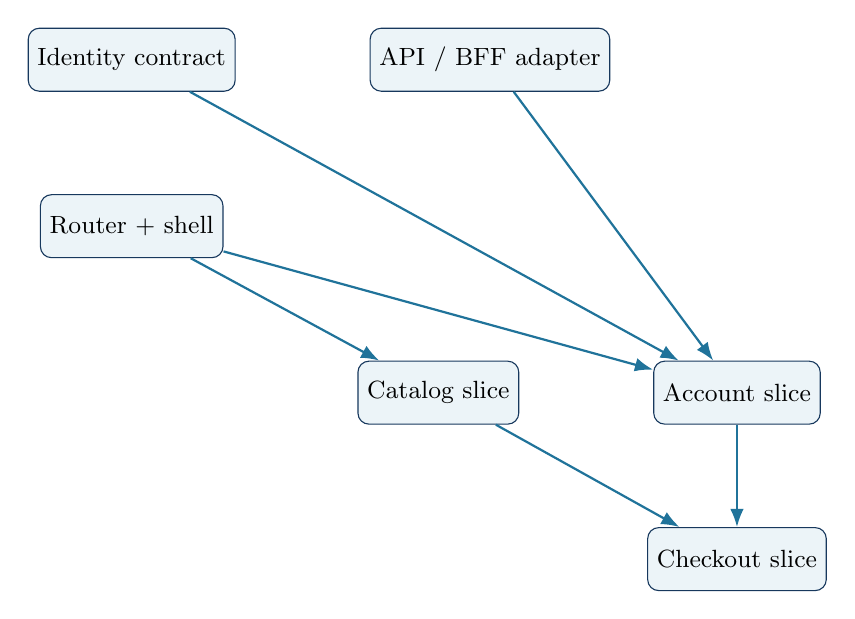
\begin{tikzpicture}[node distance=13mm and 17mm, every node/.style={font=\small}, n/.style={draw=navy,fill=pale,rounded corners,minimum height=.8cm,align=center}, a/.style={-{Latex},draw=blue,thick}]
\node[n] (identity) {Identity contract};
\node[n,right=of identity] (gateway) {API / BFF adapter};
\node[n,below=of identity] (shell) {Router + shell};
\node[n,below right=of shell] (catalog) {Catalog slice};
\node[n,right=of catalog] (account) {Account slice};
\node[n,below=of account] (checkout) {Checkout slice};
\draw[a](identity)--(account);\draw[a](gateway)--(account);\draw[a](shell)--(catalog);\draw[a](shell)--(account);\draw[a](catalog)--(checkout);\draw[a](account)--(checkout);
\end{tikzpicture}\end{center}
\noindent Arrows express \emph{prerequisite to dependent}. Keep this direction consistent in the project dependency registry.
\chapter{Migrating Cross-Cutting Concerns}
\section{Identity and session}
Do not duplicate authoritative session state in each micro-frontend. Use a trusted identity system and backend validation, consistent cookie settings and refresh/logout behavior across zones, and explicit testing of CSRF, account switching, token renewal, and expired sessions. Avoid passing raw access tokens over custom events.
\section{Routing and SEO}
Map every legacy URL to a new owner, preservation or redirect policy, and a direct-link integration test. Keep canonical metadata and sitemap decisions consistent; monitor broken deep links and search index changes. Cross-zone navigation may trigger a full document load and needs real-user performance measurement.
\section{Design and accessibility}
Publish design tokens, navigational semantics, focus-management conventions, shared error language, and a global help mechanism. Validate screen-reader and keyboard journeys that cross old/new boundary; visual similarity alone is insufficient.
\section{Data and state}
Retain backend systems of record during the UI migration unless a separate data migration is justified. Wrap legacy backend behavior behind a measured anti-corruption layer. No shared store should become an undocumented distributed transaction coordinator.
\chapter{Cutover, Rollback, and Contingency}
\section{Canary cutover card}
\begin{longtable}{p{.24\linewidth}p{.66\linewidth}}\toprule Field & Required data \\\midrule
Domain and cohort & Which routes, user segments, geography, device classes?\\
Candidate release & Immutable artifact, contract version, build/security evidence\\
Old release & Known-good route, assets, rollback manifest revision\\
Success measures & User-flow SLI, JS performance, auth error rate, operational cost\\
Abort criteria & Objective alert thresholds with on-call decision authority\\
Rollback method & Restore previous route/manifest, verify CDN convergence\\
Fallback UX & Error page or read-only experience if both versions fail\\\bottomrule\end{longtable}
\section{Cutover sequence}
\begin{enumerate}\item Freeze incompatible contract changes during initial promotion.
\item Validate source and target route permissions and backend compatibility.
\item Roll out to internal/test cohort; then controlled production cohorts.
\item Compare key SLIs and incidents to control group, adjusting for sample size.
\item On failure, execute rollback by routing change rather than re-compilation.
\item Record incident and revise fitness tests before retry.\end{enumerate}
\chapter{Migration Risks and Treatment}
\begin{longtable}{p{.3\linewidth}p{.52\linewidth}}\toprule Risk & Mitigation \\\midrule
Unclear ownership & Capability map, service catalog, accountable product owner\\
Conflicting dependency versions & Vertical-first strategy; tested sharing policy if horizontal\\
Authentication fragmentation & Central validation and cross-zone E2E test suite\\
Duplicated UX abstractions & Design tokens and stability-based component sharing\\
Regressions across routes & Contract tests plus critical cross-domain browser flows\\
Unbounded migration scope & Thin vertical slice, exit gate, rollback requirement\\
Invisible cost escalation & CDN, operational support, pipeline, and developer-time TCO\\
Backend coupling persists & Measured anti-corruption layer and explicit contract ownership\\\bottomrule\end{longtable}
\chapter{Decision and Retirement Records}
\section{Pilot completion review}
Compare the pilot with its original hypothesis, not generic success claims. Include quantitative release independence, browser performance, security findings, availability, support burden, and a user-experience narrative. Recommend expand, pause, reverse, or retain a hybrid.
\section{Legacy decommission evidence}
Require zero active route allocations, expiry of rollback obligations, removal of stale registry entries, retirement of legacy credentials, repository archival, updated incident runbooks, and a data-retention review. An extracted UI is not decommissioned merely because users no longer see it.

\refs
\end{document}
